\subsection{中介者模式(Mediator)}

模式定义一个中介对象来简化原有对象之间的交互关系,降低系统中对象间的耦合度,使原有对象之间不必相互了解。

\subsubsection{中介者模式简介}

中介者模式是一种软件设计模式,它用于将对象间的通信进行封装,使各个对象不需要直接互相引用来通信。它通过引入一个中介者对象来实现这一目的,该对象负责处理各个对象之间的通信。

中介者模式的一个常见应用场景是在多个对象之间进行通信时,避免对象之间的耦合性。例如,假设我们有两个类,一个用于表示人类,另一个用于表示车辆,它们之间需要进行通信。如果没有中介者模式,我们可能会在两个类中添加大量的代码来处理这种通信,这会导致代码难以理解和维护。

使用中介者模式,我们可以创建一个中介者类,用于处理人类和车辆之间的通信。这样,人类和车辆类就不需要直接引用对方来进行通信了,从而降低了它们之间的耦合度。

中介者模式具有以下优点:
\begin{enumerate}
\item 中介者模式可以减少对象之间的耦合度,使各个对象之间不需要直接引用来进行通信。
\item 中介者模式可以提高系统的灵活性,因为它允许在不更改对象之间的关系的情况下添加新的对象。
\item 中介者模式可以使得系统更加模块化,从而更容易实现和维护。
\end{enumerate}

中介者模式也有一些缺点,包括:
\begin{enumerate}
\item 中介者模式可能会使得系统变得过于复杂,因为它需要引入新的类来处理对象之间的通信。
\item 中介者模式可能会导致代码难以理解和维护,特别是当有大量的对象时。
\item 中介者模式可能会导致性能问题,因为它需要在多个对象之间进行额外的通信。
\end{enumerate}

\subsubsection{中介者模式在项目中的应用}

\begin{figure}[H]
    \centering
    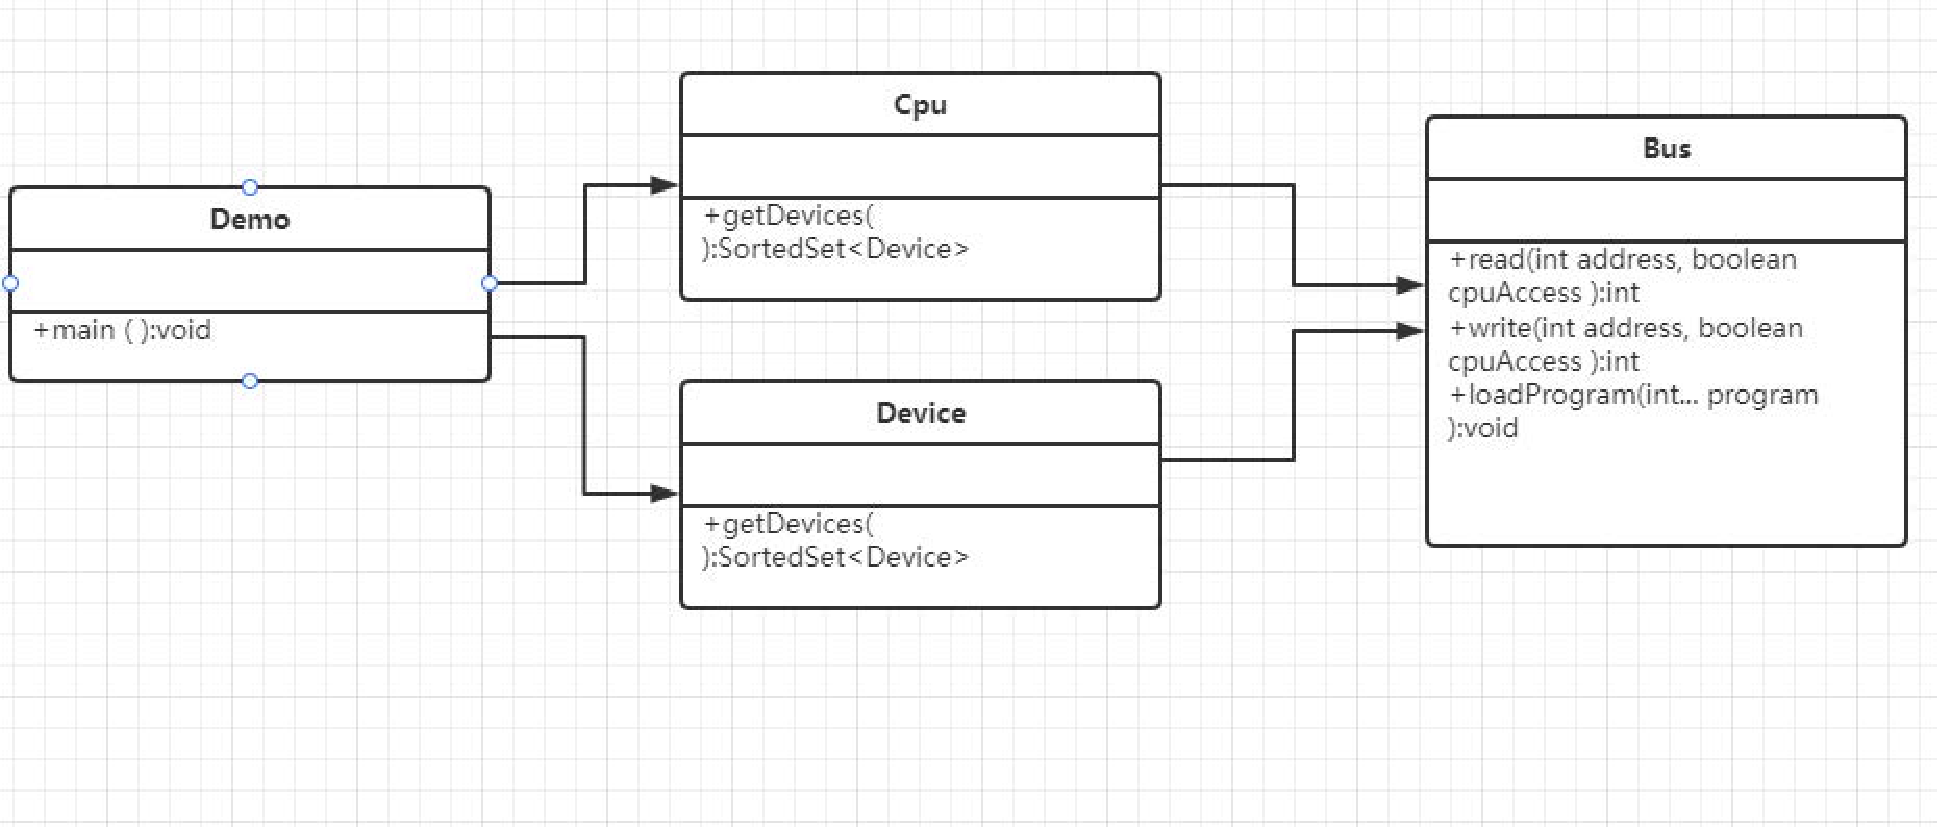
\includegraphics[width=0.9\textwidth]{figures/中介者模式.pdf}
    \caption{中介者模式在 Slow6502 中的类图}
\end{figure}

我们的项目中,Bus 就是作为 CPU 、内存和各个外设之间的中介者使用的。如果没有 Bus 作为中介者,模拟器中各个设备对象之间存在比较复杂的引用关系,导致它们之间的依赖关系结构混乱而且难以复用该对象。通过这种模式,我们使得模拟器能够方便地复用各种外设。

  